\documentclass[a4paper]{article}
\usepackage[ngerman]{babel}
\usepackage[utf8]{inputenc}
\usepackage{multicol}
\usepackage{calc}
\usepackage{ifthen}
\usepackage{geometry}
\usepackage{amsmath,amsthm,amsfonts,amssymb}
\usepackage{color,graphicx,overpic}
\usepackage{listings}
\usepackage[compact]{titlesec} %less space for headers
\usepackage{mdwlist} %less space for lists
\usepackage{pdflscape}
\usepackage{verbatim}
\usepackage[hidelinks,pdfencoding=auto]{hyperref}
\usepackage{fancyhdr}
\usepackage{lastpage}
\pagestyle{fancy}
\fancyhf{}
\fancyhead[L]{Content Verwertungsmodelle}
\fancyfoot[L]{\thepage/\pageref{LastPage}}
\renewcommand{\headrulewidth}{0pt} %obere Trennlinie
\renewcommand{\footrulewidth}{0pt} %untere Trennlinie

\pdfinfo{
    /Title (Content Verwertungsmodelle - Cheatsheet)
    /Creator (TeX)
    /Producer (pdfTeX 1.40.0)
    /Author (Robert Jeutter)
    /Subject ()
}

% This sets page margins to .5 inch if using letter paper, and to 1cm
% if using A4 paper. (This probably isn't strictly necessary.)
% If using another size paper, use default 1cm margins.
\ifthenelse{\lengthtest { \paperwidth = 11in}}
    { \geometry{top=.5in,left=.5in,right=.5in,bottom=.5in} }
    {\ifthenelse{ \lengthtest{ \paperwidth = 297mm}}
    {\geometry{top=1.3cm,left=1cm,right=1cm,bottom=1.2cm} }
    {\geometry{top=1.3cm,left=1cm,right=1cm,bottom=1.2cm} }
    }

% Redefine section commands to use less space
\makeatletter
\renewcommand{\section}{\@startsection{section}{1}{0mm}%
                                {-1ex plus -.5ex minus -.2ex}%
                                {0.5ex plus .2ex}%x
                                {\normalfont\large\bfseries}}
\renewcommand{\subsection}{\@startsection{subsection}{2}{0mm}%
                                {-1explus -.5ex minus -.2ex}%
                                {0.5ex plus .2ex}%
                                {\normalfont\normalsize\bfseries}}
\renewcommand{\subsubsection}{\@startsection{subsubsection}{3}{0mm}%
                                {-1ex plus -.5ex minus -.2ex}%
                                {1ex plus .2ex}%
                                {\normalfont\small\bfseries}}
\makeatother

% Don't print section numbers
\setcounter{secnumdepth}{0}
\setlength{\parindent}{0pt}
\setlength{\parskip}{0pt plus 0.5ex}    
% compress space
\setlength\abovedisplayskip{0pt}
\setlength{\parskip}{0pt}
\setlength{\parsep}{0pt}
\setlength{\topskip}{0pt}
\setlength{\topsep}{0pt}
\setlength{\partopsep}{0pt}
\linespread{0.5}
\titlespacing{\section}{0pt}{*0}{*0}
\titlespacing{\subsection}{0pt}{*0}{*0}
\titlespacing{\subsubsection}{0pt}{*0}{*0}

\begin{document}

\begin{multicols*}{2}
  % multicol parameters
  % These lengths are set only within the two main columns
  %\setlength{\columnseprule}{0.25pt}
  \setlength{\premulticols}{1pt}
  \setlength{\postmulticols}{1pt}
  \setlength{\multicolsep}{1pt}
  \setlength{\columnsep}{2pt}
  \raggedright

  \section{Mobile Geräte - Smartphones}
  Was sollte ein Endgerät können?
  \begin{itemize*}
    \item Content wiedergeben
    \item $\leftrightarrow$ Mensch-Maschine-Schnittstelle
    \item $\rightarrow$ Laden/Zuführen des Content bzw. -Daten
  \end{itemize*}
  %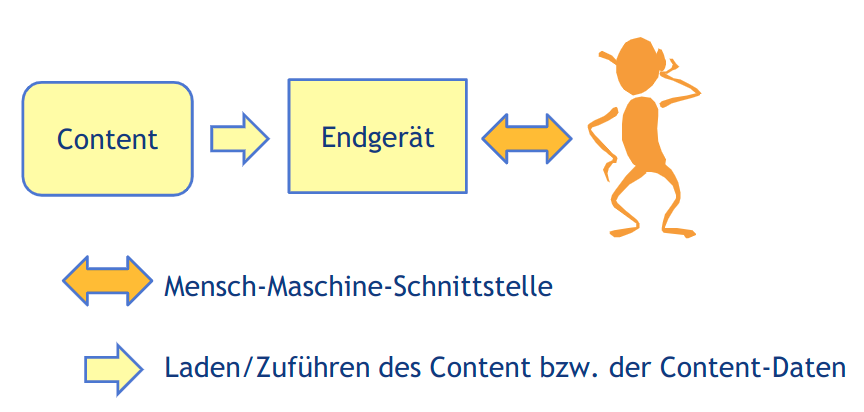
\includegraphics[width=.5\linewidth]{Assets/ContentVerwertungsmodelle-content.png}

  \begin{itemize*}
    \item Mobile Endgeräte ermöglichen die ...
    \begin{itemize*}
      \item mobile Nutzung von Content
      \item mobile elektronische Kommunikation
      \item Verarbeitung der Nutzer- und Gerätemobilität
    \end{itemize*}
    \item Was ist nicht mobil? tragbar aber nicht mobil nutzbar
  \end{itemize*}

  Was macht ein Endgerät intelligent (= smart)?
  \begin{itemize*}
    \item enthält ein(en) freiprogrammierbarer Rechner
    \item hat einen Internet-Zugang
    \item kann Content erstellen und im Internet bereitstellen
    \item kann Content aus dem Internet laden
    \item kann Content weiterverarbeiten
  \end{itemize*}

  \subsection{Entwicklung des Mobilfunks bis LTE}
  \begin{itemize*}
    \item 1918-1926: anfang bei der Reichsbahn in Deutschland
    \item Erste Generation
    \begin{itemize*}
      \item A-Netz 1958 (teuer, schwer, in Bereiche unterteilt)
      \item B-Netz 1972
      \item C-Netz 1985 (cellulär)
    \end{itemize*}
    \item GSM ab 1992, 2. Generation (2G), D und E-Netz
    \begin{itemize*}
      \item GPRS (General Packet Radio)
    \end{itemize*}
    \item UMTS, 3. Generation (3G) ab ca 2000
    \item LTE ab 2010
  \end{itemize*}

  \subsection{5G Technology}
  \begin{itemize*}
    \item Milimeter Waves, 30-600GHz
    \begin{itemize*}
      \item greater spectrum of communication, less interference
      \item high frequenzy cannot travel through walls
    \end{itemize*}
    \item Small Cell (Networks)
    \begin{itemize*}
      \item more small base stations
    \end{itemize*}
    \item Massive MIMO
    \begin{itemize*}
      \item multiple input multiple output
      \item more ports
    \end{itemize*}
    \item Beamforming
    \begin{itemize*}
      \item traffic signaling
      \item focus stream to single user
    \end{itemize*}
    \item Full Duplex
  \end{itemize*}

  \subsection{Historische Geräte - Meilensteine}
  \begin{itemize*}
    \item erste Handy: Motorola DynaTAC, 1983
    \item erste GSM Handy für Massen: Nokia 1011, 1992
    \item erste WAP-Handy: Nokia 7110, 1999
    \item erste App-Handy: iPhone, 2007
  \end{itemize*}

  \subsection{Die nahe Zukunft - Wearables}
  \begin{itemize*}
    \item Wear OS  by Google
    \item Samsung Gear S3
    \item Apple Watch 4 mit EKG
  \end{itemize*}

  \newpage
  \section{Mobile Geräte - Betriebssysteme}
  \subsection{Was ist ein Betriebssystem?}
  Zusammenstellung von Computerprogrammen, die Systemressourcen eines Computers wie Arbeitsspeicher, Festplatten, Ein- und Ausgabegeräte verwaltet und diese Anwendungsprogrammen zur Verfügung stellt.

  Bildet dadurch Schnittstelle zwischen den Hardwarekomponenten und der Anwendungssoftware des Benutzers.
  % [Andrew S. Tanenbaum: Moderne Betriebssysteme](Andrew S. Tanenbaum: Moderne Betriebssysteme. 3., aktualisierte Auflage, Pearson Studium, ISBN 978-3-8273-7342-7)
  % [http://de.wikipedia.org/wiki/Betriebssystem](http://de.wikipedia.org/wiki/Betriebssystem)

  \subsection{PDA- und Smartphone-Betriebssysteme}
  \begin{itemize*}
    \item Android ... (Marktanteil 2020 weltweit: 72,3%)
    \item Apple iOS ... (Marktanteil: 27,0%)
    \item Windows 10 Mobile ... (Marktanteil: 0,1%)
    \item BlackBerry OS und BlackBerry 10 ... (Marktanteil: 0,01%)
    \item \href{http://de.wikipedia.org/wiki/Tizen}{Tizen}: freies OS für Samsungs Smartwatches
    \item \href{http://de.wikipedia.org/wiki/Ubuntu_Touch}{Ubuntu Touch}: mobile Benutzeroberfläche für Ubuntu
    \item Kein Betriebssystem: Java Micro Edition (Java ME) ...
  \end{itemize*}

  MIDP-Java ME (kein Betriebssystem)
  \begin{itemize*}
    \item Überblick
    \begin{itemize*}
      \item Mobile Information Device Profile ist ein Profil der Java Micro Edition, das speziell auf die Fähigkeiten kleiner Mobilgeräte wie Mobiltelefon oder PDA ausgelegt wurde. Es umfasst daher Funktionen zur Ansteuerung und Abfrage von Einhandtastaturen, Miniaturbildschirmen, flüchtigem und nicht-flüchtigem Speicher im Kilobyte-Bereich etc.
      \item MIDP-Applikationen heißen MIDlets
    \end{itemize*}
    \item 1. Version 2000; 2. 2002; 3. 2009
    \item BlackBerry setzte bis Version 7 auf MIDP 2.0
  \end{itemize*}

  \subsection{Symbian}
  \begin{itemize*}
    \item Handy-OS hat seine Ursprünge in 32-Bit-EPOC-Plattform von Psion; diese wurde in einem 1998 gegründetem Konsortium mit dem Namen Symbian von den Mobilfunkunternehmen Ericsson, Motorola, Nokia und Psion eingesetzt und weiterentwickelt.
    \item Symbian Ltd. wurde vollständig durch Nokia übernommen und in eine gemeinnützige Organisation, die Symbian Foundation, überführt. Nokia erwarb im Dezember 2008 sämtliche Rechte und übertrug sie an die Symbian Foundation. Diese erklärte Symbian im Februar 2010 zur Open Source-Lösung.
    \item Unterstützung durch Nokia Ende 2012 komplett eingestellt
    \item Symbian hat vieles mit Desktop-Betriebssystemen gemein, z. B. präemptives Multitasking, Multithreading und Speicherschutz.
  \end{itemize*}

  \subsection{BlackBerry}
  \begin{itemize*}
    \item Das Blackberry OS ist ein proprietäres, kostenlos nutzbares Multitasking-Betriebssystem für Smartphones. Es wird von dem Unternehmen Blackberry für dessen Geräte der Marke Blackberry entwickelt. Apps können im zugehörigen Blackberry-World-Store erworben werden. Der Nachfolger von Blackberry OS heißt Blackberry 10.
    \item Blackberry OS wurde inzwischen durch Blackberry 10 auf QNX-Basis ersetzt. Im August 2013 hat BlackBerry mit dem 9720 noch ein Einsteiger-Smartphone mit BlackBerry OS 7.1 vorgestellt.
    \item Es ist in C++ programmiert und bietet eine Java-Umgebung (J2ME - MIDP) mit speziellen Schnittstellen zum Betrieb von Programmen. Drittentwicklern steht eine spezielle Programmierschnittstelle zur Verfügung. Integraler und bekanntester Bestandteil der Funktionalität sind die E-Mail-Funktionen der Plattform.
    \item Laut Gartner war es mit 17,5 Prozent Marktanteil im Jahr 2010 eines der bedeutendsten Betriebssysteme für Mobiltelephone
  \end{itemize*}

  \subsection{Windows Phone, Windows 10 Mobile}
  \begin{itemize*}
    \item Entwicklung von Windows Phone wurde Anfang September 2010 abgeschlossen
    \item Im Gegensatz zum Vorgänger Windows Phone 7 basiert Windows Phone 8 nicht länger auf Windows CE, sondern demselben Windows-NT-Kernel wie Windows 8 und Windows RT.
    \item Windows Phone 8 wurde am 20. Juni 2012 auf der Windows Phone Summit in San Francisco vorgestellt.
    %\item [http://de.wikipedia.org/wiki/Microsoft_Windows_Phone_8](http://de.wikipedia.org/wiki/Microsoft_Windows_Phone_8)
    \item Windows 10 Mobile
    \begin{itemize*}
      \item Nachfolger von Windows Phone 8.1
      \item Wurde stark an die Desktop-Version angelehnt
      \item Weiterentwicklung wurde 2017 beendet
      \item Supportende: 14. Januar 2020
      %\item https://de.wikipedia.org/wiki/Microsoft_Windows_10_Mobile
    \end{itemize*}
  \end{itemize*}

  \subsection{iOS}
  \begin{itemize*}
    \item iOS ist von Apple entwickeltes mobiles Betriebssystem für iPhone, iPad, iPod touch und Apple TV der 2. und 3. Generation
    \item iOS nur auf eigener Hardware von Apple eingesetzt
    \item basiert auf einem "Mac OS X"-Kern bzw. Darwin-Betriebssystem, welches wiederum auf einen Unix-Kern zurückgeht
    \item ursprüngliche Betriebssystem wurde am 9. Januar 2007 zusammen mit dem iPhone auf der MacWorld Conference and Expo vorgestellt. iPhone OS (iOS) unterstützte zu diesem Zeitpunkt noch keine Apps von externen Entwicklern.
    \item Am 6. März 2008 veröffentlichte Apple das SDK für iOS, um Drittentwicklern die Möglichkeit zu geben, Apps für iOS entwickeln zu können.
    \item Die damit entwickelten Apps lassen sich ausschließlich im ebenfalls mit iPhone OS 2.0 neu eingeführten App Store veröffentlichen.
    %\item Versionen [http://de.wikipedia.org/wiki/Apple_iOS\#Versionen](http://de.wikipedia.org/wiki/Apple_iOS\#Versionen)
    \item UI Toolkit ist Cocoa Touch im Unterschied zum OS X's Cocoa. Das UI ist nicht mit OS X kompatibel.
    %\item Das Bedienkonzept von iOS ist möglichst einfach gehalten. Somit beschränkt es sich fast ausschließlich auf den Home-Bildschirm. iOS wird fast ausschließlich über den Multitouchbildschirm gesteuert, nur das Sperren und Ausschalten des Geräts wird mit dem Lockbutton ausgelöst, und das Beenden von Anwendungen (genannt Apps) mit dem Homebutton. Dieser kann das Gerät ebenso wie der Lockbutton aus dem Standby-Modus aufwecken. iOS ist darauf ausgelegt mit allen anderen Apple-Produkten zusammenzuarbeiten. Es unterstützt Multi-Touch mit bis zu fünf Fingern. Multitouch wird teilweise zur Gestensteuerung verwendet, so lassen sich beispielsweise Apps durch Gesten schließen oder wechseln.
  \end{itemize*}

  \subsection{Android}
  \begin{itemize*}
    \item sowohl Betriebssystem als auch Software-Plattform für mobile Geräte wie Smartphones, Netbooks und Tablet-Computer, die von der Open Handset Alliance entwickelt wird. Basis ist der Linux-Kernel. Es handelt sich um freie Software, die quelloffen entwickelt wird.
    \item 2005 kaufte Google das 2003 von Andy Rubin gegründete Unternehmen Android
    \item Ursprünglich ausschließlich zur Steuerung von Digitalkameras gedacht
    \item Seit dem 21. Oktober 2008 ist Android offiziell verfügbar
    \item Als erstes Gerät mit Android als Betriebssystem kam am 22. Oktober 2008 das HTC Dream unter dem Namen T-Mobile G1 in den USA auf den Markt. Dass bereits dieses erste Gerät auf das Global Positioning System (GPS) zugreifen konnte und mit Bewegungssensoren ausgestattet war, gehörte zum Konzept von Android.
    %\item [Oberfläche](http://de.wikipedia.org/wiki/Android_%28Betriebssystem%29\#Oberfl.C3.A4che_und_Bedienung)
    \item Architektur: baute anfangs auf dem Linux-Kernel 2.6 auf, ab Android 4.x auf einen Kernel der 3.x-Serie.
    %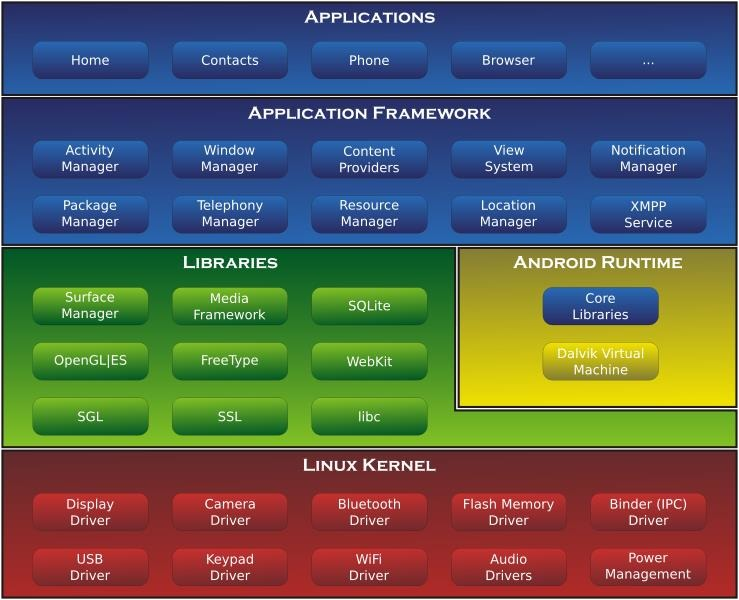
\includegraphics[width=.5\linewidth]{Assets/ContentVerwertungsmodelle-Android-Architektur.jpg}
    %\item [Versionen](https://de.wikipedia.org/wiki/Liste_von_Android-Versionen)
    \item Java
    \begin{itemize*}
      \item Anwendungen in der Regel in Java geschrieben
      \item Java-Laufzeitumgebung von Android basiert auf Dalvik Virtual Machine, ähnelt funktional der normalen Java-VM. Wesentlicher Unterschied virtuelle Prozessorarchitektur.
      \item Java-VM basiert auf Kellerautomaten; Dalvik-VM ist Registermaschine
      \item Da das Prozessormodell des Kellerautomaten besonders einfach ist, wird es üblicherweise für die Übersetzerzwischensprache verwendet.
    \end{itemize*}
  \end{itemize*}

  \subsection{Fuchsia von Google}
  \begin{itemize*}
    \item nicht auf einen Linux-Kernel basierend
    \item Echtzeitbetriebssystem basiert auf Mikrokernel Zircon
    \item Läuft auf verschiedenen Mobiltelefonen und PCs
    \item unklar, ob und wann Fuchsia Android ersetzen soll
  \end{itemize*}

  \subsection{Wear OS}
  \begin{itemize*}
    \item Wear OS von Android abgeleitet und speziell für Smartwatches und andere Wearables
    \item am 18. März 2014 erstmal präsentiert. Laut Hersteller bietet es Google-Now-Funktionen im Gehäuse einer Armbanduhr.
    \begin{itemize*}
      \item Mit Google-Now erhält man Karten mit hilfreichen Informationen für den Tagesablauf
      \item Seit 2017 ist Android Wear 2.0 verfügbar.
      \item Seit 2018 unbenannt in "Wear OS by Google"
    \end{itemize*}
  \end{itemize*}
  %\item https://de.wikipedia.org/wiki/Wear_OS

  \newpage
  \section{Apps - Entwurf und Programmierung}
  \subsection{Was ist eine App?}
  \begin{itemize*}
    \item steht für application und bezeichnet Anwendungssoftware
    \item dienen der Lösung von Anwenderproblemen
    \item grenzt sich von Systemsoftware und systemnaher Unterstützungssoftware ab
  \end{itemize*}
  %[http://de.wikipedia.org/wiki/Anwendungssoftware](http://de.wikipedia.org/wiki/Anwendungssoftware)

  \subsection{App-Grundtypen}
  \subsubsection{Native App}
  \begin{itemize*}
    \item speziell für ein Betriebssystem ausschließlich mit hierfür breitgestellten SDK (System Development Kit) entwickelt wurde. Wird über App-Stores verbreitet und auf dem Endgerät installiert.
    \item Vorteil: native App kann die über das jeweilige Betriebssystems angebotenen Hardware-Ressourcen optimal nutzen. kann sehr performant und Ressourcen-sparend sein.
    \item Nachteil: müssen für jedes Betriebssystem getrennt entwickelt werden. Die Entwicklungskosten sind sehr hoch
  \end{itemize*}

  \subsubsection{Web-App}
  \begin{itemize*}
    \item Web-App läuft komplett im Browser, wird als Web-Seite vom Web-Server geladen. Nutzt HTML, CSS und JavaScript
    \item Vorteil: HTML, CSS und JS auf allen Betriebssystemen standardisiert, laufen Web-Apps auf allen Systemen. Dies reduziert die Entwicklungskosten.
    \item Nachteil: HTML, CSS und JS muss vom Browser interpretiert werden. Performanz gering. Browser kann nicht auf alle Hardware-Ressourcen (wie z.B. Kamera und Datei-System) zugreifen. Kann nicht über App-Stores verbreitet werden.
  \end{itemize*}

  \subsubsection{Hybrid}
  \begin{itemize*}
    \item native App, die für Darstellung der Oberfläche Browser-Komponente nutzt. Der größte Teil der App ist in HTML, CSS und JS. Nativer Code über JS der Oberfläche zugänglich, ermöglicht Zugriff auf native Gerätefunktionen.
    \item Vorteil: kann alle über das jeweilige Betriebssystems angebotenen Hardware-Ressourcen nutzen. Kann über App-Stores verbreitet werden. Die Oberfläche und die Interaktionslogik sind für alle Betriebssysteme gleich. Dies reduziert die Entwicklungskosten.
    \item Nachteil: HTML, CSS und JS müssen vom Browser interpretiert werden. Daher ist die Performanz/Reaktionszeit der Oberfläche oft gering.
  \end{itemize*}

  \subsection{User-Interface (UI) Prototype Design}
  \begin{itemize*}
    \item Wireframes (Drahtgerüst) oder Mock-Ups (Attrape) werden dazu benutzt, um einen sehr frühen konzeptuellen (nicht funktionsfähigen) Prototypen eines App-Frontends darzustellen. Navigation und Nutzerführung und wesentliche Inhaltsbereiche sollten Teil dieses Skeletts sein.
    \item Im Gegensatz zu statischen Wireframes ermöglichen dynamische Wireframes die Navigation zwischen den einzelnen Ansichten.
    %\item Beispiele
    %  \item [Balsamiq](http://www.balsamiq.com)
    %  \item [Proto.io](http://www.proto.io)
    %  \item [InVision](http://www.invisionapp.com)
    %  \item [Fluid UI](https://www.fluidui.com)
    %  \item [UXPin](http://www.uxpin.com)
    %  \item [Pencil](http://pencil.evolus.vn/)
    %\end{itemize*}
  \end{itemize*}

  \subsection{Entwicklungsumgebungen}
  \begin{itemize*}
    \item IDEs für Apps
    \item Xcode von Apple (Swift)
    \item Android Studio (Java)
    \item Visual Studio IDE Community 2019
    \item Visual Studio Code (Universal IDE)
    \item Cross-Plattform
    \item React Native (by Facebook)
    \item Xamarin (Mono, C\#)
    \item Flutter (by Google, in Dart)
    \item Hybrid
    \item Apache Cordova (PhoneGap)
    \item Ganz anders
    \item App Inventor (online grafisch)
    \item Angular (by Google)
  \end{itemize*}

  \section{Was ist (mobile) Content?}
  \subsection{Was ist Content?}
  \begin{itemize*}
    \item seit 1990 im Zusammenhang mit neuen Medien und später Internet als Synonym für (digitalisierten) Medieninhalt
    \item Medieninhalte werden von Infrastruktur eines Mediums abgegrenzt. Der Content von YouTube ist beispielsweise nicht die Plattform als ganzes, sondern die Gesamtheit der abrufbaren Videos mit ihren Beschreibungen und Nutzerkommentaren.
    \item Content ist das, was für den Konsumenten einen Wert/Nutzen darstellt
    \item Content ist Information die über ein Medium (den Kanal) übermittelt wird
  \end{itemize*}

  Was passiert mit Content? Content wird ...
  \begin{itemize*}
    \item produziert,
    \item gespeichert,
    \item übertragen
    \item und konsumiert
  \end{itemize*}

  \subsubsection{Content-Typen bzw. Medientypen}
  Die Daten werden als Datei gespeichert bzw. als Stream übertragen. Der Internet Media Type, auch MIME-Type (nach der Spezifikation Multipurpose Internet Mail Extensions) oder Content-Type (nach dem Namen des Feldes), klassifiziert die Content-Daten.

  Der Internet Media Type besteht aus zwei Teilen: der Angabe eines Medientyps und der Angabe eines Subtyps(z.B. image/png).

  Es gibt folgende Medientypen:
  \begin{description*}
    \item[application] uninterpretierte binäre Daten, Mischformate oder Informationen
    \item[audio] für Audiodaten
    \item[example] Beispiel-Medientyp für Dokumentationen
    \item[image] für Grafiken
    \item[message] für Nachrichten, beispielsweise message/rfc822
    \item[model] Daten, mit mehrdimensionale Strukturen
    \item[multipart] für mehrteilige Daten
    \item[text] für Text
    \item[video] für Videomaterial
  \end{description*}

  \subsection{Was ist mobiler Content?}
  \begin{itemize*}
    \item kann auf mobilen Endgerät mobil genutzt
    \item für die mobile Nutzung speziell aufbereitet (umgewandelt)
    \item bei Bildern möglicherweise die Größe angepasst
    \item Nicht jeder Content (z.B. Spielfilme) ist für mobile Nutzung
  \end{itemize*}

  \subsection{User-generated Content (UGC)}
  \begin{itemize*}
    \item Content, der nicht vom Anbieter der Plattform, sondern von dessen Nutzern erstellt wird
    \item Konsumenten sind gleichzeitig Produzenten, auch Prosumer genannt
    \item Häufig eine Erscheinungsform von Crowdsourcing
  \end{itemize*}

  \subsection{Open Data}
  \begin{itemize*}
    \item freie Verfügbar- und Nutzbarkeit von Daten (bzw. Content), typischerweise öffentlicher bzw. staatlicher Einrichtungen
    \item föderung vorteilhafter Entwicklungen z.B. Open Government
    \item Offene Daten sind sämtliche Datenbestände, die im Interesse der Allgemeinheit der Gesellschaft ohne jedwede Einschränkung zur freien Nutzung, zur Weiterverbreitung und zur freien Weiterverwendung frei zugänglich gemacht werden.
    \item z.B. Lehrmaterial, Geodaten, Statistiken, Verkehrsinformationen,...
    \item IdR verzicht auf Copyright, Patente oder andere proprietäre Rechte
  \end{itemize*}

  \newpage

  \section{Urheberrecht im Wandel der Zeit}
  \subsection{Vor dem Urheberrecht}
  \begin{itemize*}
    \item Bücher einzeln hergestellt, verkauft und bezahlt
    \item Schriftsteller, Maler, ...wie Handwerker behandelt
    \item wurden nur für Ihre Arbeit entlohnt
    \item Ein Buch durfte abgeschrieben werden
    \item Rang eines Künstlers nach handwerklichen Fertigkeiten
    \item durch Buchdruck viel einfacher Kopien herzustellen
    \item Drucker erbaten von der Obrigkeit Sonderrechte
    \item Die Obrigkeit hatte ein gleiches Interesse (Zensur)
    \item Privilegien dienten dem Schutz der Verleger zur Sicherung ihres Absatzes
  \end{itemize*}

  \subsection{Anfänge des Urheberrechts ...}
  \begin{itemize*}
    \item 1710, England: Statute of Anne
    \begin{itemize*}
      \item Recht des Autors an seinem Werk
      \item Zuvor Recht bei Verleger
      \item Zweck war Förderung der Bildung
      \item exklusive Druckrecht den jeweiligen Autoren oder den Erwerbern dieses Rechts für die im Gesetz bestimmte Zeiteingeräumt wurde.
      \item für neue Werke begrenzte das Gesetz die Schutzfrist auf 14 Jahre. Nach deren Ablauf stand dem lebenden Autor eine Verlängerung um weitere 14 Jahre zu.
    \end{itemize*}
    \item 1837, Preußen: Schutz von 10 Jahren
    \item 1845 Schutz auf 30 Jahre nach dem Tod des Autors verlängert
    \item 1870 wurde im Norddeutschen Bund ein allgemeiner Urheberrechtsschutz eingeführt, den das Deutsche Reich 1871 übernahm.
    \item 1965, BRD deutsche Urheberrechtsgesetz (UrhG)
    \begin{itemize*}
      \item Urheberfrist auf 70 Jahre nach dem Tod des Urhebers angehoben (Vorreiter)
      \item Privatkopie wieder legalisiert,
    \end{itemize*}
  \end{itemize*}

  \subsection{Neue Entwicklungen}
  \begin{itemize*}
    \item 1996 durch Weltorganisation für geistiges Eigentum der WIPO-Urheberrechtsvertrag und der WIPO-Vertrag über Darbietungen und Tonträger unterzeichnet.
    \begin{itemize*}
      \item Anpassung nationaler Urheberrechtsgesetze an die Anforderungen digitaler Netzmedien
      \item Vervielfältigungsrecht gestärkt und Speichern von Werken im Computer ausdrücklich subsumiert
      \item Recht auf Zugänglichmachung. Übertragung und Anbieten im Internet nur mit Zustimmung der Urheber zulässig
      \item Juristischer Schutz technischer Schutzmaßnahmen. Komponenten, deren Zweck es ist, Kopierschutzmechanismen der Rechteinhaber zu umgehen sind verboten. Es ist auch verboten, die Wirkungsweise dieser Komponenten zu beschreiben, so dass sie nachgebaut werden können
      \item Juristischer Schutz von Copyright Management Information. Auch die Veränderung, Fälschung oder Löschung von Informationen, die Urheber oder Konsumenten identifizieren oder erlaubte Nutzungsformen festlegen, sind verboten.
    \end{itemize*}
    \item 1998, USA$\rightarrow$ Digital Millennium Copyright Act
    \item 2001, EU $\rightarrow$WIPO-Vertrag in Richtlinie 2001/29/EG
    \item 2003, Deutschland folgt mit Urheberrechts-Novelle
    \begin{itemize*}
      \item "Wirksame technische Maßnahmen zum Schutz..."
      \item "...dürfen ohne Zustimmung des Rechtsinhabers nicht umgangen werden,..."
      \item ... durch Zugangskontrolle,... Verschlüsselung, Verzerrung oder sonstige Umwandlung
    \end{itemize*}
    \item 2008 der "2. Korb" der Novelle
    \begin{itemize*}
      \item Erhalt der Privatkopie, außer rechtswidriges Angebot
      \item Es gibt keine Durchsetzung der Privatkopie gegen Kopierschutz
    \end{itemize*}
  \end{itemize*}

  \subsection{Schranken des Urheberrechts}
  Ausgleich zwischen Interessen des Urhebers, dem ausschließliches Nutzungsrecht eingeräumt ist und gegenläufigen Interessen (der Nutzer).

  Systematische Schranken zugunsten einzelner Nutzer, der Kulturwirtschaft sowie der Allgemeinheit.

  Darunter Erlaubnis der Vervielfältigung zu eigenem Gebrauch, die Entlehnungsfreiheit (z.B. Zitate) und Gestattung der öffentlichen Wiedergabe im Lehrbetrieb.
  %[http://de.wikipedia.org/wiki/Schranken_des_Urheberrechts](http://de.wikipedia.org/wiki/Schranken_des_Urheberrechts)

  \subsection{Urheberrecht versus Copyright}
  \begin{itemize*}
    \item Copyright des U.S. Rechtssystems: ökonomischen Aspekte im Mittelpunkt
    \item Urheberrecht, welches Schöpfer und seine ideelle Beziehung zum Werk in den Mittelpunkt
    \item Copyright bis 1989 in den USA explizit angemeldet werden und erlosch 75 Jahre später
    \item jetzt neue Werke ein Schutz bis 70 Jahre nach dem Tod des Urhebers bzw. 95 Jahre für Firmen (Copyright Term Extension Act)
    \item Anmeldung des Copyrights bei der Library of Congress nicht erforderlich, kann aber vorteilhaft
  \end{itemize*}

  \subsection{Fair Use}
  \begin{itemize*}
    \item bestimmte, nicht autorisierte Nutzungen von geschütztem Material, sofern sie der öffentlichen Bildung und der Anregung geistiger Produktionen dienen.
    \item Die Doktrin erfüllt eine vergleichbare Funktion wie die Schrankenbestimmungen des kontinentaleuropäischen Urheberrechts.
    \item Im amerikanischen Rechtsraum gestattet Fair Use neben Zitaten etwa auch Parodien auf ein urheberrechtlich geschütztes Werk aber nicht Satiren.
  \end{itemize*}

  \subsection{Creative Commons}
  \begin{itemize*}
    \item Werke eines Urhebers sind normalerweise urheberrechtlich geschützt.
    \item Urheber kann entscheiden, dass er Werke anderen Menschen zur Verfügung stellt
    \item CC: englisch für schöpferisches Gemeingut, Kreativallmende ist eine gemeinnützige Organisation, die 2001 in den USA gegründet wurde
    \item veröffentlicht verschiedene Standard-Lizenzverträge
    \item drei Entscheidungsfragen:
    \begin{itemize*}
      \item Nennung des Urhebers vorgeschrieben?
      \item kommerzielle Nutzung erlaubt?
      \item Veränderungen erlaubt?
    \end{itemize*}
    \item Daraus ergaben sich zwölf Lizenzmöglichkeiten.
    \item Bsp: Public Domain: nein, ja, ja
    \item Bsp: GPL: nein, ja, nur mit gleicher Lizenz
  \end{itemize*}

  \subsubsection{Rechtemodule}
  \begin{tabular}{l | l}
    Kurz & Name des Moduls                                     \\\hline
    by   & Namensnennung (englisch:Attribution)                \\
    nc   & Nicht kommerziell (Non-Commercial)                  \\
    nd   & Keine Bearbeitung ( No Derivatives)                 \\
    sa   & Weitergabe unter gleichen Bedingungen (Share Alike)
  \end{tabular}

  \newpage
  \section{Geschäftsmodelle und Cloud-Dienste}
  \subsection{Geschäftsmodelle mit Content}
  \begin{itemize*}
    \item Geschäftsmodell beschreibt modellhaft, wie ein Unternehmen Werte auf einem Markt erzielt
    \item Verwertungsmodell ist ein Geschäftsmodell, für geistiges Eigentum
    \item Content basiert auf geistigem Eigentum.
    \item Geschäftsmodell durch drei Hauptkomponenten charakterisiert:
    \begin{itemize*}
      \item Architektur von Produkten, Dienstleistungen und Informationsflüssen, mit beteiligten Wirtschaftsakteure und deren Rollen
      \item potentiellen Nutzen, den das Unternehmen für die verschiedenen Wirtschaftsakteure bietet
      \item Erlösmodell, zeigt aus welchen Quellen und wie sich das Unternehmen finanziert
    \end{itemize*}
    \item Content-Geschäftsmodelle variieren bei:
    \begin{itemize*}
      \item Datei-Download
      \item Online-Konsum/Streaming
      \item Peer-to-peer (P2P) und Superdistribution
      \item Download mit DRM (Verleih, Abo)
    \end{itemize*}
  \end{itemize*}

  \subsection{Abgrenzung von öffentlichen Gütern}
  Content-Geschäftsmodelle beruhen darauf, dass Rivalität und Ausschließbarkeit bei der Nutzung von Content ermöglicht werden kann.

  Außschließbarkeit \& Rivalität
  \begin{tabular}{p{4cm} | p{4cm} }\hline
    Individualgut oder privates Gut (Kleidung)               & Allmendegut oder Quasikollektivgut (öffentliche Straßen)                  \\\hline
    Klubkollektivgut oder natürliche Ressource (Feuerschutz) & Öffentliches Gut oder reines Kollektivgut (Rechtsordnung, Währungssystem) \\\hline
  \end{tabular}

  \subsection{Wert \& Kosten von Content}
  Soll ein spezielles Content-Geschäftsmodell erfolgreich sein, muss es die drei verschiedene Wertebegriffe Warenwert, Gebrauchswert und Tauschwert in Einklang bringen und dabei auch das bestehende Wertverständnis der Konsumenten beachten.

  Stückkostendegression bei Content

  \subsection{Erlösmodelle und Erlösformen}
  Die Erlöse für Content bestimmen den Wert und die Nachhaltigkeit eines Geschäftsmodells
  \begin{itemize*}
    \item Direkt vs Indirekt
    \item Nutzungsabhängig vs Unabhängig
    \item von Unternehmen vs Staat
  \end{itemize*}
  \begin{tabular}{ l|l|l  }
    Nutzungsabhängig & Einmalig          & Wiederkehrend \\\hline
    Pay-per-use      & Lizenzgebühren    & Abonnement    \\
    Pay-per-time     & Abschlussgebühren & Grundgebühren \\
    Transaktion      & App Kauf          & Werbung
  \end{tabular}


  \subsection{Einordnung von Cloud-Diensten}
  \begin{multicols*}{2}
    nach Dienst
    \begin{itemize*}
      \item On-Premise
      \item Colocation
      \item Hosting
      \item IaaS (Infrastructure)
      \item PaaS (Platform)
      \item SaaS (Software)
    \end{itemize*}
    \columnbreak
    nach Angebot
    \begin{itemize*}
      \item Data
      \item Application
      \item Databases
      \item Operating System
      \item Virtualization
      \item Physical Servers
      \item Network \& Storage
      \item Data Center
    \end{itemize*}
  \end{multicols*}

  \subsection{Cloud Markt 2019}
  \begin{itemize*}
    \item EC2 von Amazon Web Services (Elastic Cloud Compute)
    \item Virtualisierte Server
    \item Flexible Preismodelle
  \end{itemize*}

  \section{Distribution über AppStore und Google-Play}
  Überblick
  \begin{itemize*}
    \item Ohne App Store
    \item Mit App Store
    \item App Store Guidelines
    \item Einreichung bei Apple
    \item Jailbreak
    \item Einreichung bei Google Play
    \item Und bei Microsoft
  \end{itemize*}

  \section{Distribution über AppStore und Google-Play}
  \subsection{Wie geht es ohne?}
  \begin{itemize*}
    \item Software häufig vom Entwickler zum Nutzer vertrieben
    \item Bestellung und Bezahlung vom Nutzer direkt an Entwickler
    \item Entwickler hatten große Freiheiten
    \item Bezahlung der Software immer anders
  \end{itemize*}

  \subsection{Apple App Store}
  Apple führt den zentralen App Store ab iOS 2.0 ein. Alle Entwickler müssen ihre Apps hierüber vertreiben. Alle Apps werden von Apple geprüft. Der Entwickler ist sehr eingeschränkt. Der Entwickler erhält 70\% des Verkaufspreises. Direktvertrieb nur für zeitlich limitierte Test-Versionen.
  \begin{itemize*}
    \item App muss Apple's App Store Guidelines befolgen
    \item Was Apple zu Beispiel nicht haben möchte
    \begin{itemize*}
      \item unfertige apps oder häufige abstürze
      \item kein Klon bekannter/beliebter Apps
      \item gleiche Features/Content bieten wie Webseite
      \item keine ähnlichkeit zu Apple Produkten/Werbung
      \item kein pornographischer Inhalt
    \end{itemize*}
  \end{itemize*}

  \subsection{Einreichung bei Apple im Überblick}
  \begin{itemize*}
    \item Um App über App Store verbreiten zu können, benötigt Entwickler Apple Developer Account und muss Mitglied im iOS Developer Programm sein.
    \item Für die Einreichung wird benötigt:
    \begin{itemize*}
      \item Eindeutige App ID
      \item Distribution Certificate \& Private Key
      \item Distribution Provisioning Profile
      \item Optional: Push Notification Certificate
      \item Icons und Loading Screens
    \end{itemize*}
    \item Test einer iOS App mit TestFlight
  \end{itemize*}

  \subsection{iOS Jailbreak}
  \begin{itemize*}
    \item nicht-autorisierte Entfernen von Nutzungsbeschränkungen
    \item Hersteller sperren bestimmte Funktionen serienmäßig
    \item Apple striktes "Closed World"-Geschäftsmodell
    \item bei Geräten mit Linux/Android eher "Rooten"
    \item modifiziert, um Zugriff (Root) auf interne Funktionen sowie das Dateisystem zu erhalten
    \item Anschließend wird Softwareverwaltung aufgespielt
    \item Da iOS auf dem Unix-artigen Betriebssystem Darwin basiert, erhält der Benutzer mit dem Jailbreak gleichzeitig Administrator-Zugriff auf ein vollwertiges Unix-Betriebssystem.
  \end{itemize*}
  %[http://de.wikipedia.org/wiki/Jailbreak_(iOS)](http://de.wikipedia.org/wiki/Jailbreak_(iOS))

  \subsection{Einreichung Google Play im Überblick}
  \begin{itemize*}
    \item Android Apps (*.apk) können auch direkt an die App-Nutzer verteilt werden. Google Play ist nicht der einzige "App Store” für Android Apps. Google Play ist aber bei den meisten Android-Geräten vorinstalliert.
    \item Registrierung bei der Google Play Developer Console
    \item Einreichung Google Play im Detail
    \begin{itemize*}
      \item Im Detail gibt es einiges zu beachten:
      %\item [How to Upload Android Apps to Google Play Store](http://www.youtube.com/watch?v=GCmXjdp--HM)
    \end{itemize*}
  \end{itemize*}

  \subsection{Microsoft?}
  Microsoft hat sich an Apple orientiert. Auch bei Microsoft geht nichts am Store vorbei.
  % \item https://docs.microsoft.com/de-de/windows/uwp/publish/

  \newpage
  \section{Payed-Content und In-App-Payment}
  \subsection{Bezahlsysteme}
  Bezahlsysteme für Content sind spezialisierte Vermittler und Dienstleister. Sie stehen zwischen Käufer und Content-Anbieter.

  \subsection{Bezahlsysteme und Payed-Content}
  \begin{itemize*}
    \item Bezahlsysteme ermöglichen erst Payed-Content
    \item Da bei Content Transaktionshöhe oft sehr gering, können Transaktionen beim Bezahlsystem gebündelt werden, um Kosten für den Content-Anbieter zu senken.
    \item Neue Abrechnungsmodelle (z.B. Abonnement) können vom Bezahlsystem angeboten werden.
    \item technischer Aufwand bei Content-Anbieter kann reduziert werden
    \item Mangel an Vertrauen in kleine Content-Anbieter Problem. Durch zwischengeschaltetes bekanntes Bezahlsystem Bedenken der Käufer reduziert
  \end{itemize*}

  \subsection{Abrechnungsmethoden}
  \begin{description*}
    \item[Vorkasse/Überweisung] Bevor der Content-Anbieter den Content ausliefert, muss der Käufer den vollen Betrag überweisen. Diese Abrechnungsmethode bietet dem Händler maximale Sicherheit, da der Kunde eine Überweisung kaum stornieren kann.
    \item[Rechnung] Käufer zahlt erst nach Erhalt der Ware. Bei der Abrechnung von Content wird diese Methode nicht eingesetzt.
    \item[Lastschrift] Der Käufer autorisiert den Content-Anbieter, den festgelegten Rechnungsbetrag vom Käuferkonto abzubuchen. Kann storniert werden, keine Zahlungsgarantie. kostengünstigsten Abrechnungsmethoden.
    \item[Kreditkarte] Käufer teilt dem Content-Anbieter seine Kreditkartendaten mit, die von diesem zur Abrechnung mit dem zwischengeschalteten Kreditkartenunternehmen benutzt werden. keine Zahlungsgarantie
    \item[Inkasso per Telefon] Rechnungsbetrag über die Telefonrechnung beglichen. Entweder über den Anruf einer Mehrwertnummer oder das Senden einer SMS-Nachricht (sog. Premium-SMS) an eine spezielle Mobilfunknummer. Es fallen nicht nur die normalen Verbindungskosten an, sondern darüber hinaus zusätzliche Entgelte, die die jeweilige Telefongesellschaft an den Content-Anbieter weiterleitet. zählt zu den teuersten Methoden, oft weniger als 50\% übrig.
    \item[Freischaltkarten] Vor dem eigentlichen Kauf von Content muss der Kunde zuerst eine Rubbelkarte erwerben. Durch Eingabe von Buchstaben-Ziffern-Kombination autorisiert der Käufer Zahlungen. nahezu einzige Möglichkeit, Content vollständig anonym zu bezahlen
  \end{description*}

  \subsection{Ausgewählte Bezahlsysteme}
  \begin{description*}
    \item[Paypal] kann Zahlungen anderer PayPal-Nutzer entgegen nehmen. Möchte man eine  Peer-to-Peer-Zahlung in PayPal durchführen, muss man nur die E-Mail-Adresse des Zahlungsempfängers wissen. Im PayPal-System gibt man dann diese Adresse, den Betrag und einen Betreff ein und löst per Klick die Transaktion aus. Der Empfänger wird von PayPal per E-Mail über den Eingang einer Zahlung informiert.
    \item[Click\&Buy] (gibt es nicht mehr) Im Unterschied zu den kontenbasierten Systemen ist click\&buy ein Inkasso/Billing-System, welches auf Content beschränkt ist. Die einzelnen Rechnungsbeträge werden gesammelt und am Monatsende per Lastschrift abgebucht bzw. der Kreditkarte belastet und an die jeweiligen Händler überwiesen.
    \item[Paysafecard] vertreibt Freischaltkarten für Zahlungen im Internet. Prinzip analog zu Prepaid-Karten für Mobiltelefone.
    \item[Amazon Payments] Amazon wickelt inzwischen auch für andere Online-Shops Zahlungen ab. Der Käufer nutzt hierbei zur Zahlung seine Daten aus dem Amazon-Account.
  \end{description*}

  \columnbreak
  \subsection{Apples App Store ist ein Bezahlsystem}
  \begin{itemize*}
    \item App Store ist sein eigenes Bezahlsystem aus iTunes
    \item für Inbetriebnahme eines iPhones ist ein Account im App Store zwingend notwendig. Später auch Anmeldung ohne Kreditkarte möglich
    \item Entwickler muss sich nicht um die Abwicklung der Bezahlung kümmern.
    \item Viele Apple Nutzer vertrauen Apple. Hat der Nutzer einmal ein App bezahlt, ist der Vorgang bei der nächsten App der Gleiche.
    \item App-Entwickler erhalten 70\% des Netto-Verkaufspreises von Apple
  \end{itemize*}

  \subsection{In-App-Payment}
  \begin{itemize*}
    \item Seit iOS 3.0 ermöglicht Apple allen App-Entwicklern Payed-Content über ihre App zu verkaufen
    \item Entwickler dürfen Content in ihren Apps allerding nur über Apple verkaufen
    \item physische Produkte nicht erlaubt abzurechnen
    \item keine Erotik und anderer Apple untersagten Inhalte
    \item Entwickler können Content-Shop und -Player in App verbinden
    \item Entwickler können bestimmte Funktionen ihrer App gegen Bezahlung freischalten lassen
    \item Entwickler können Online-Dienste und Zugang zu Datenbanken abrechnen lassen
  \end{itemize*}

  \subsection{Consumable und Non-Consumable}
  \begin{description*}
    \item[Consumable Products] der sich verbraucht z.B. VoIP Gesprächsminuten
    \item[Non-Consumable Products] der erhalten bleibt und auf allen Geräten eines Nutzers verfügbar ist z.B. E-Books
  \end{description*}

  \begin{tabular}{ p{4cm} |c|c}
                                     & Non-consu. & Consumable \\\hline
    Wie oft kaufen                   & einmal     & mehrmals   \\
    mit Beleg                        & jedes mal  & einmalig   \\
    Synchronisiert mit Nutzergeräten & ja         & nein       \\
    Wiederhergestellung möglich      & ja         & nein
  \end{tabular}

  \subsection{Abonnements (subscription)}
  \begin{description*}
    \item[Non-renewable] Erlauben den Verkauf von Dienstleistungen mit einer begrenzten Laufzeit. Die App muss dafür sorgen, dass der Zugang auf allen Geräten eines Nutzers möglich ist. Ablauf und Dauer des Abo muss die App (bzw. der Server) durchsetzen.
    \item[Auto-renewable] Analog zu non-consumable products sind diese Abos unbegrenzt auf alle Geräten eines Nutzers verfügbar. Es können regelmäßig neue Inhalte geliefert werden, zu denen der Nutzer Zugang erhält, während das Abo aktiv ist. Diese Abos haben ein Ablaufdatum, welches automatisch durch das System verlängert wird, sofern der Nutzer nicht dies ablehnt.
  \end{description*}

  \subsection{Google Play Billing Library}
  \begin{itemize*}
    \item Der Google-Play-Store hat die Funktionalität, die Apple bietet, ebenfalls zur Verfügung. Dort wird es über die Google Play Billing Library umgesetzt.
    \item Android-Nutzer sind allerdings von Google nicht wie die Apple-Nutzer von Anfang an zum Bezahlen erzogen worden. Das macht es für Content-Anbieter schwieriger.
    \item Erst seit Mitte 2013 sind flächendeckend Google-Play- Store Rubbelkarten im Handel verfügbar. Dies ermöglicht es nun auch Jugendlichen, ohne Kreditkarte, Apps und Content bei Google Play zu bezahlen.
  \end{itemize*}
  %[Use the Google Play Billing Library](https://developer.android.com/google/play/billing)

  \newpage
  \section{Digital Rights Management}
  Verschlüsselung von Content
  \begin{itemize*}
    \item Content-Daten werden verschlüsselt
    \item Anbieter verteilt nur verschlüsselte Nutzdaten
    \item Verschlüsselung/Entschlüsselung mit gleichen Schlüssel
    \item Schlüssel wird getrennt und geheim übermittelt
  \end{itemize*}

  \subsection{Symmetrische Verschlüsselung}
  \begin{itemize*}
    \item Einfacher Algorithmus: Bitweise Addition (XOR)
    \begin{itemize*}
      \item Beispiel: Verschlüsselung
      \begin{itemize*}
        \item Content = 11 = 1011
        \item Schlüssel = 9 = 1001
        \item Daten = 1011 XOR 1001 = 0010 = 2
      \end{itemize*}
      \item Beispiel: Entschlüsselung
      \begin{itemize*}
        \item Verschl. Content = 2 = 0010
        \item Schlüssel = 9 = 1001
        \item Content = 0010 AND 1001 = 1011
      \end{itemize*}
    \end{itemize*}
    \item XOR: One-Time-pad, Block Schlüssel
    %\includegraphics[width=.5\linewidth]{Assets/ContentVerwertungsmodelle-sym-verschlüsselung-xor.png)
    \item Blockweise Verschlüsselung
    \begin{itemize*}
      \item XOR kann in der Praxis nur einmalig angewendet werden (Klartext-Angriff gelingt)
      \item Gute sym. Verfahren (AES) ermöglichen wiederholte Anwendung des Schlüssels
      \item Blocklänge und Schlüssellänge z.B. 128/256 Bit
      %\includegraphics[width=.5\linewidth]{Assets/ContentVerwertungsmodelle-sym-verschlüsselung-block.png)
    \end{itemize*}
  \end{itemize*}

  \subsection{AES - Advanced Encryption Standard}
  \begin{itemize*}
    \item Standard nach dem Verfahren von Rijndael
    \item 128 Bit Blocklänge mit 128, 192 oder 256 Bit Schlüssel
    \item Realisierung in Hardware und Software sehr schnell
    \item Je nach Schlüssellänge: 10, 12 oder 14 Runden
    \item Frei von Patenten und unentgeltlich nutzbar
    %\item Details: https://en.wikipedia.org/wiki/Advanced_Encryption_Standard
  \end{itemize*}

  \subsection{Kontrolle über den Schlüssel}
  \begin{itemize*}
    \item Schlüssel wird im Endgerät kontrolliert
    \item DRM-Controller kontrolliert Verwendung des Schlüssels
    \item Schlüssel muss vor dem Nutzer verborgen bleiben
    \item DRM-Controller darf nicht vom Nutzer verändert werden
    %\includegraphics[width=.5\linewidth]{Assets/ContentVerwaltungsmodelle-Schlüsselkontrolle.png)
  \end{itemize*}

  \subsection{Lizenzen (oder Rechteobjekte)}
  \begin{itemize*}
    \item Lizenzen enthalten Schlüssel und Rechtebeschreibung
    \item Verschlüsselte Content-Daten sind ohne Lizenz wertlos
    \item Rechtebeschreibung legt die zulässige Nutzungsart (z.b. abpielen) und Nutzungsdauer fest
    \item Verschlüsselte Nutzdaten können kopiert werden
    \item Lizenzen an Endgerät gebunden (keine Weitergabe)
  \end{itemize*}

  \subsection{Public-Key-Kryptographie}
  \begin{itemize*}
    \item Es gibt zwei Schlüssel (=Schlüsselpaar)
    \item Was mit dem einen verschlüsselt wird kann nur mit dem anderen entschlüsselt werden (=asymmetrisch)
    \item ein Schlüssel öffentlich: Public Key
    \item anderer Schlüssel privat: Private Key
  \end{itemize*}

  \subsection{Anwendungen bei DRM}
  \begin{itemize*}
    \item Geheime Übertragung des CEK (Cont. Encry. Key)
    \item Endgerät fordert von einem Lizenz-Server den passenden Schlüssel für die Content-Daten an.
    \item Lizenz-Server verschlüsselt den CEK  mit dem öffentlichen Schlüssel des Endgerätes
  \end{itemize*}
  %\includegraphics[width=.5\linewidth]{Assets/ContentVerwertungsmodelle-CEK-übertragung.png)

  \subsection{Allgemeine Anwendungen}
  \begin{itemize*}
    \item Verschlüsselte E-Mail oder SSL
    \begin{itemize*}
      \item E-Mail Sender verschlüsselt Nachricht mit öffentlichen Schlüssel des Empfängers
      \item asymmetrische Verfahren langsam $\rightarrow$ Inhalt mit schnellen symmetrischen Algorithmus verschlüsselt. Der symmetrische Schlüssel wird mit dem öffentlichen Schlüssel des Empfängers verschlüsselt. (=hybrid)
    \end{itemize*}
    \item Digitale Signatur
    \begin{itemize*}
      \item Integrität von Nachrichten und Authentizität von Kommunikationspartner sicherstellen
      \item Ausgetauschte Dokumente nicht verändern
      \item vereinfacht: Sender überträgt Dokument doppelt, einmal unverschlüsselt, zweites mal mit seinem privaten Schlüssel
      \item Besser: Sender verschlüsselt mit privaten Schlüssel nur eine Prüfsumme des Dokumentes
    \end{itemize*}
  \end{itemize*}

  \subsection{Authentizität durch Zertifikate}
  \begin{itemize*}
    \item öffentliche Schlüssel alleine nicht trauen
    \item Von offiziellen Instanz (CA - Certification Authority) ausgestellte Zertifikate bieten Abhilfe
    \item Was ist ein Zertifikat (nach X.509)?
    \begin{itemize*}
      \item öffentlicher Schlüssel und
      \item Datensatz über den Besitzer des Schlüssel
      \item beides zusammen von einer CA digital signiert
      \item das Zertifikat der CA kann beigefügt sein
    \end{itemize*}
    \item Zertifikatsketten: Aussteller des Zertifikates besitzt ein eigenes Zertifikat
  \end{itemize*}

  \subsection{Kryptogr. Hash-Funktion (Streuwertfunktion)}
  \begin{itemize*}
    \item Funktion, die zu Eingabe aus großer Quellmenge eine Ausgabe aus kleineren Zielmenge erzeugt
    \item \textbf{Kollisionsfreiheit} nicht effizient möglich, zwei Quellelemente mit demselben Hash-Wert zu finden
    \item \textbf{Unumkehrbarkeit} Zur Funktion gibt es keine effizient berechenbare Umkehrfunktion, mit der es möglich wäre, für ein gegebenes Zielelement ein passendes Quellelement zu finden
  \end{itemize*}
  %\includegraphics[width=.5\linewidth]{Assets/ContentVerwertungsmodelle-krypto-hash.png)

  \subsection{Sicherung der Integrität \& Authentizität}
  \begin{itemize*}
    \item ... der Lizenz durch digitale Signatur
    \item mit Private Key des Lizenz-Servers wird ein über die Rechte und Schlüssel errechneter Hash-Wert verschlüsselt
    %\includegraphics[width=.5\linewidth]{Assets/ContentVerwertungsmodelle-lizenz-digitale-signatur.png)
  \end{itemize*}

  \subsection{RSA Verfahren (Rivest, Shamir, Adleman)}
  \begin{itemize*}
    \item Multiplikation ist einfach. Umkehrung (Faktor.) schwer
    \item zwei ~gleich lange Primzahlen: $p$ und $q$ ($p=11, q=13$)
    \item Berechne $n = p*q$ ($n = 143$)
    \item Berechne $\phi(n) = (p-1)*(q-1)$ ($=120$)
    \item Wähle $e$ (23) mit $ggT(e,\phi(n)) = 1$
    \item Berechne $d$ so, dass $e * d \equiv 1\ mod \phi(n)$ gilt, $e * d = k * \phi(n) + 1$ ($d = 47$ mit $k = 9$)
    \begin{itemize*}
      \item Public Key: $(n,e) (143, 23)$
      \item Private Key: $(n,d) (143, 47)$
      \item Verschlüsselung mit Public Key:
      \begin{itemize*}
        \item $C = K^e \text{ mod } n$
        \item $2 = 723 \text{ mod } 143$
      \end{itemize*}
      \item Entschlüsselung mit Private Key:
      \begin{itemize*}
        \item $K = C^d \text{ mod } n$
        \item $7 = 2^{47} \text{ mod } 143$
      \end{itemize*}
      \item Damit n im praktischen Anwendungsfall nicht in p und q faktorisiert werden kann, muss n aktuell eine 1024 bis 2048 bit lange Zahl sein !!
    \end{itemize*}
    \item $e = 65537$ fast immer gleich, damit öffentlich
  \end{itemize*}

  \subsection{Referenz-Modell für DRM-Systeme}
  \begin{itemize*}
    \item Download des Contents
    \item Content wird geöffnet
    \item DRM-Controller fordert eine Lizenz an
    \item Lizenz wird geöffnet
    \item der private Geräteschlüssel wird benötigt
    \item Nutzungszähler werden geprüft und angepasst
    \item Entschlüsselter Content wird decodiert
  \end{itemize*}
  %\includegraphics[width=.5\linewidth]{Assets/ContentVerwertungsmodelle-DRM-Modell.png)


  \subsection{Zusammenfassung}
  \begin{itemize*}
    \item Content ist symmetrisch verschlüsselt
    \begin{itemize*}
      \item Content-Daten sind ohne Schlüssel (CEK) wertlos
      \item im unversch. Teil steht Adresse des Lizenz-Servers
    \end{itemize*}
    \item Schlüssel wird in der Lizenz transportiert
    \begin{itemize*}
      \item Lizenz enthält Rechtebeschreibung
      \item Rechte werden im DRM-Controller ausgewertet
    \end{itemize*}
    \item Asymmetrische Kryptographie
    \begin{itemize*}
      \item Nachrichten von beiden Seiten signiert
      \item Zertifikate werden eingesetzt
      \item Schlüssel (CEK) in der Lizenz wird vom Server mit dem öffentlichen Schlüssel des Endgerätes verschlüsselt
      \item privater Endgeräteschlüssel ist Sicherheitsanker
    \end{itemize*}
  \end{itemize*}

  \newpage
  \section{Mobile Entrepreneurship}
  \subsection{Unternehmertum}
  Unternehmertum/Gründertum/Gründerkultur, beschäftigt sich als wirtschaftswissenschaftliche Teildisziplin mit Gründungsgeschehen oder Gründung von neuen Organisationen als Reaktion auf identifizierte Möglichkeiten und als Ausdruck spezifischer Gründerpersönlichkeiten, die ein persönliches Kapitalrisiko tragen.
  %[Wikipedia](https://de.wikipedia.org/wiki/Unternehmertum)

  \subsection{Zielgruppe und Einschränkung}
  \begin{itemize*}
    \item Einzelpersonen und Mini-Teams (2-3 Personen)
    \item Noch keine Unternehmer
    \item Haben eine erste Version einer App entwickelt
    \item Einschränkungen: Kein Ersatz für eigenen Business-Plan
  \end{itemize*}

  \subsection{Fragen vor Gründung}
  \begin{itemize*}
    \item Bin ich ein/e Unternehmer/in?
    \item Möchte ich Geld verdienen?
    \item Möchte ich neue Kunden gewinnen?
    \item Was ist mein Geschäftsmodell?
    \item Welche Rechtsform?
    \item Wie komme ich an nötiges Kapital?
  \end{itemize*}

  \subsection{Geschäftsmodell (Empfehlung)}
  \begin{itemize*}
    \item Wo kommen 1000 bis 3000 Euro im Monat her?
    \begin{itemize*}
      \item Tipp: Wenige, dafür zahlungskräftige Kunden!
    \end{itemize*}
    \item Entwickeln Sie zuerst ein B2B-Geschäftsmodell
    \begin{itemize*}
      \item B2B: Business-to-Business (Firmen sind Kunden)
      \item B2C: Business-to-Consumer (zu Privatpersonen)
    \end{itemize*}
    \item Beispiel für B2B-Geschäftsmodell
    \begin{itemize*}
      \item App findet für Allergiker die richtige Zeit zum Joggen
      \item Mögliche Firmen: Krankenkassen, Sportartikel-Hersteller ...
      \item White-Label-Konzept, um App mehreren Kunden zu "verkaufen"
      \item Betreiben Sie benötigte Server gegen Gebühr selbst
    \end{itemize*}
  \end{itemize*}

  \subsection{Wie komme ich an das nötige Kapital?}
  \begin{itemize*}
    \item Durststrecke bis zum ersten B2B-Kunden selbst finanzieren
    \item Crowdfunding oder Crowdinvesting
  \end{itemize*}

\end{multicols*}

\end{document}